\documentclass[a4paper,10pt]{article}

\usepackage[utf8]{inputenc} % allow utf-8 input
\usepackage{hyperref}       % hyperlinks
\usepackage{url}            % simple URL typesetting
\usepackage{booktabs}       % professional-quality tables
\usepackage{amsfonts}       % blackboard math symbols
\usepackage{nicefrac}       % compact symbols for 1/2, etc.
\usepackage{microtype}      % microtypography
\usepackage{graphicx}       % include graphics
\usepackage{subcaption}     % subfigures
\usepackage{float}          % placement of floats
\usepackage{fancyhdr}       % head notes and foot notes
\usepackage{bbm}            % Nice symbols
\usepackage{mathtools}      % Math tools like operators
\usepackage{listings}       % Write code in a listing
\usepackage[left=2cm,right=2cm,top=3cm,bottom=3cm]{geometry}

\graphicspath{ {assets/} }

% Operators
\DeclarePairedDelimiter\abs{\lvert}{\rvert} % abs
\DeclarePairedDelimiter\norm{\lVert}{\rVert} % norm
\DeclareMathOperator*{\argmax}{arg\,max} % argmax
\newcommand{\p}{\mathbbm{P}} % Big P for probabilties
\newcommand{\pd}[2]{\frac{\partial #1}{\partial #2}}  % Partial derivative

% To prevent the tilde from being printing above with lstlisting
\lstset{
    literate={~} {$\sim$}{1},
    showstringspaces=false,
    numbers=left,
    breaklines=true
}

% Sections naming conventions
\renewcommand{\thesection}{\arabic{section}}
\renewcommand{\thesubsection}{(\alph{subsection})}
\renewcommand{\thesubsubsection}{\roman{subsubsection}.}

% Head and foot notes
\pagestyle{fancy}
\fancyhf{}
\lhead{Louis MARTIN}
\rhead{Big Data Processing and Analytics: Assignment 1}
\rfoot{Page \thepage}

\begin{document}

\title{Big Data Processing and Analytics: Assignment 1}
\author{Louis MARTIN\\
\href{mailto:louis.martin@student.ecp.fr}{\tt louis.martin@student.ecp.fr}}

\maketitle

In this assignment we are going to create an inverted index on a corpus
including the complete works of William Shakespear, Mark Twain and Jane Austen
using Hadoop's MapReduce framework.

\section{Setup}
\subsection{System specifications}

\begin{itemize}
    \item \textbf{Operating system}:\\
    Ubuntu 16.04 (Native)
    \item \textbf{System specifictations}:\\
    Model: Dell Inspiron 17R 5720\\
    Processor: i5-3210M\\
    Cores: 2\\
    Threads: 4\\
    Ram: 8 GB\\
    Storage: 256GB SSD (MLC)
    \item \textbf{Java version}:\\
    openjdk version "1.8.0\_121"\\
    OpenJDK Runtime Environment (build 1.8.0\_121-8u121-b13-0ubuntu1.16.04.2-b13)\\
    OpenJDK 64-Bit Server VM (build 25.121-b13, mixed mode)
    \item \textbf{Haddop version}:\\
    Hadoop 2.7.3\\
    Subversion https://git-wip-us.apache.org/repos/asf/hadoop.git -r baa91f7c6bc9cb92be5982de4719c1c8af91ccff\\
    Compiled by root on 2016-08-18T01:41Z\\
    Compiled with protoc 2.5.0\\
    From source with checksum 2e4ce5f957ea4db193bce3734ff29ff4\\
    This command was run using /usr/local/hadoop/share/hadoop/common/hadoop-common-2.7.3.jar\\

\end{itemize}

Hadoop was installed using \href{https://www.digitalocean.com/community/tutorials/how-to-install-hadoop-in-stand-alone-mode-on-ubuntu-16-04}{this tutorial} and configured using \href{https://hadoop.apache.org/docs/stable/hadoop-project-dist/hadoop-common/SingleCluster.html}{this tutorial}.


\subsection{Configuration}
The configuration comes from the \href{https://hadoop.apache.org/docs/stable/hadoop-project-dist/hadoop-common/SingleCluster.html}{official documentation} for a single Hadoop node cluster.
The following configuration files allows Hadoop and YARN to run in a pseudo-distributed mode.
\begin{itemize}
    \item \textbf{core-site.xml:}
    \lstinputlisting[firstline=19, lastline=24, language=xml]{assets/hadoop_conf/core-site.xml}
    \item \textbf{hdfs-site.xml:}
    \lstinputlisting[firstline=19, lastline=24, language=xml]{assets/hadoop_conf/hdfs-site.xml}
    \item \textbf{mapred-site.xml:}
    \lstinputlisting[firstline=19, lastline=24, language=xml]{assets/hadoop_conf/mapred-site.xml}
    \item \textbf{yarn-site.xml:}
    \lstinputlisting[firstline=15, lastline=29, language=xml]{assets/hadoop_conf/yarn-site.xml}
    \item \textbf{Commands to set up HDFS and YARN:}
    \begin{lstlisting}[language=bash]
      # Format the filesystem
      hdfs namenode -format
      # Start HDFS
      start-dfs.sh

      # Create directories to execute MapReduce jobs
      hdfs dfs -mkdir /user
      hdfs dfs -mkdir /user/louis

      # Put the data in HDFS
      hdfs dfs -put ~/dev/bdpa/a1/data data

      # Start YARN Ressource manager
      start-yarn.sh
    \end{lstlisting}
\end{itemize}


\subsection{Bugs encountered}
I encountered a bug while running the MapReduce jobs where I would be logged out and all my processes would be killed with no warning.
After investigation, I found that \href{https://bugs.launchpad.net/ubuntu/+source/procps/+bug/1610499}{this is a known bug referenced here} and caused by /bin/kill in ubuntu 16.04.

I compiled propcps-3.3.10 from source to solve the problem as indicated in launchpad but to no avail.
\begin{lstlisting}[language=bash]
  # (1) download the sourcecode
  sudo apt-get source procps

  # (2) install dependency
  sudo apt-get build-dep procps

  # (3) compile procps
  cd procps-3.3.10
  sudo dpkg-buildpackage
\end{lstlisting}


I tried another solution from \href{http://stackoverflow.com/questions/38419078/logouts-while-running-hadoop-under-ubuntu-16-04}{this stackoverflow thread} but it didn't work either.
The supposed fix was to add
\begin{lstlisting}
  [login]
  KillUserProcesses=no
\end{lstlisting}
to \lstinline{/etc/systemd/logind.conf} and restart.

As I could find a solution I had to cope with the problem and restart all the
services every once in a while.

\section{Inverted index}
\subsection*{Workflow}
In order to facilitate compiling the $.java$ files into $.jar$ files, I created
the $compile.sh$ script which takes as input parameter the name of the main class of the $.java$ file.
\\Example: \lstinline{./compile.sh StopWords}.
\\ \textbf{compile.sh}:
\lstinputlisting[language=bash]{assets/code/compile.sh}

\subsection*{Assumptions}
After investigating the results of the different mapreduce jobs, I chose to define
all of the following characters as words separators in addition to space
\\ \textbf{Separators:} .,?!"'()[]\$*-\_;:$|$

Even if I lost some hyphenated words and contractions like "first-born" or "He's", the gain in
coherence and clarity was worth the hassle.

\subsection{Stop words\\
(30) Run a MapReduce program to identify stop words (words with frequency $> 4000$)
for the given document corpus. Store them in a single csv file on HDFS
(stopwords.csv). You can edit the several parts of the reducers’ output after the job
finishes (with hdfs commands or with a text editor), in order to merge them as a single
csv file.}


Based on the wordcount example from the \href{https://hadoop.apache.org/docs/stable/hadoop-mapreduce-client/hadoop-mapreduce-client-core/MapReduceTutorial.html}{official documentation},
we implement a MapReduce program that retrieves all the stopwords from a corpus,
i.e. it retrieves the words with wordcount greater than 4000.
\\The file is \textbf{StopWords.java}
\begin{itemize}
  \item \textbf{Mapper}:\\
  This mapper splits a string into words (tokens) and outputs one (key, value) pair
  for each word with the key being the word and the value equal to 1.
  \lstinputlisting[firstnumber=18, firstline=18, lastline=34, language=java]{assets/code/StopWords.java}
  \item \textbf{Reducer}:\\
  The reducers, simply counts the number of occurences of each key writes it to
  the output file only if its count is greater than 4000.
  \lstinputlisting[firstnumber=36, firstline=36, lastline=53, language=java]{assets/code/StopWords.java}
  \item \textbf{Job configuration}:\\
  The MapReduce task is set to write the output as a csv file.
  We can set the number of reducers, combiner and compression through command line
  arguments.
  \lstinputlisting[firstnumber=55, firstline=55, lastline=101, language=java]{assets/code/StopWords.java}
  \item \textbf{Script running the experiments}:\\
  We run the set of experiments with the \textbf{run\_stopwords.sh} script.
  This script executes the StopWords MapReduce task with different parameters
  and merges all the outputs into a csv file in HDFS.
  \lstinputlisting[language=bash]{assets/code/run_stopwords.sh}
  \item \textbf{Results}:
  Here is an extract of the output csv:
  \lstinputlisting[firstnumber=10, firstline=10, lastline=20]{assets/code/stopwords.csv}
\end{itemize}


\subsubsection{(10) Use 10 reducers and do not use a combiner. Report the execution time.}
The running time with 10 reducers is \textbf{126 seconds}.
\begin{figure}[H]
  \centering
  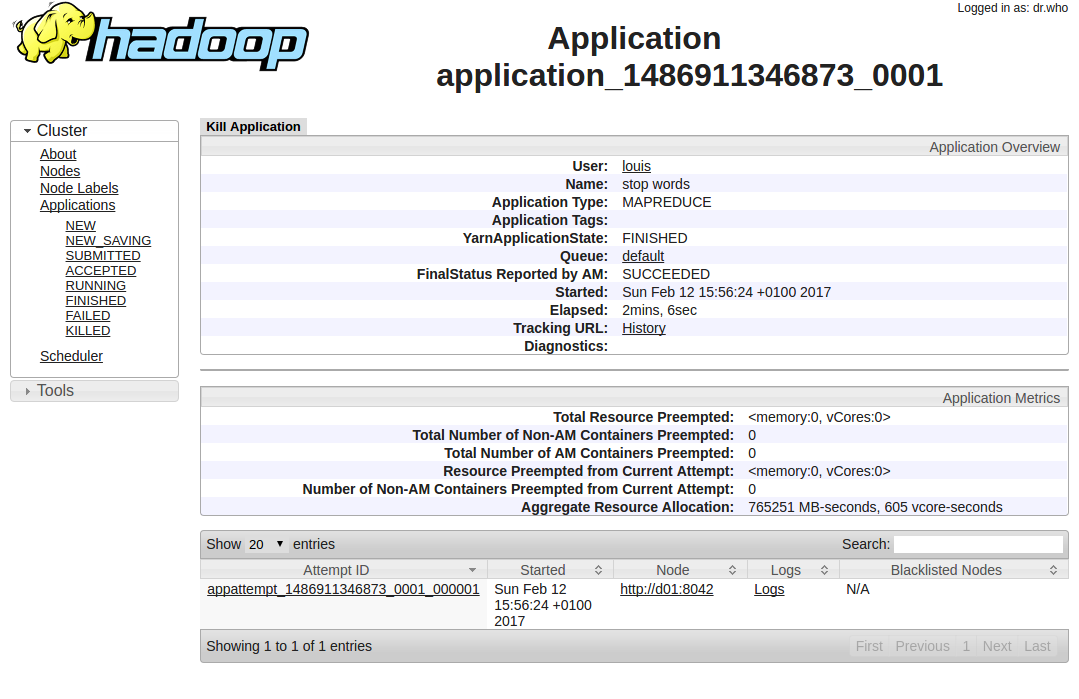
\includegraphics[width=.6\textwidth]{stopwords_10_reducers.png}
\end{figure}

\subsubsection{(10) Run the same program again, this time using a Combiner. Report the
execution time. Is there any difference in the execution time, compared to
the previous execution? Why?}
The running time with 10 reducers and combiner is \textbf{105 seconds}.
The running time is lower with the combiner. Indeed the combiner takes the output
of each mapper separately and tries to reduce as many (key, value) pairs coming
from this specific mapper as it can.
Combining the data like this will lower the load for the reducers, and all the
intermediary steps between the mappers and the reducers such as network transfer
(does not occur for a pseudo-distributed cluster), sorting all the (key, value)
pairs, assigning them to each reducer...
\begin{figure}[H]
  \centering
  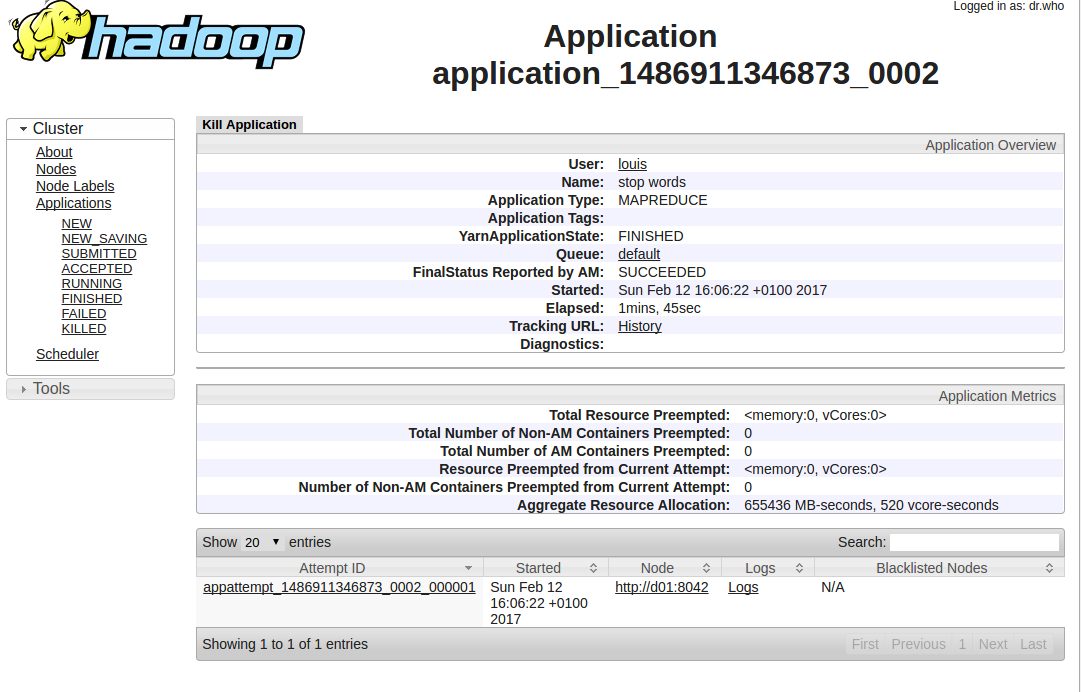
\includegraphics[width=.6\textwidth]{stopwords_10_reducers_1_combiner.png}
\end{figure}

\subsubsection{(5) Run the same program again, this time compressing the intermediate
results of map (using any codec you wish). Report the execution time. Is there
any difference in the execution, time compared to the previous execution?
Why?}
Compression compresses the data between the mappers and the reducers.
The running time with 10 reducers, combiner and compression is \textbf{125 seconds}.
The running time increased. This can be explained by the fact that compression adds
an additional overhead and its benefit is not used for a single node cluster!
Indeed compression is often used to reduce network transfer times, which does not
occur here as all the mappers and reducers are on the same device.
\begin{figure}[H]
  \centering
  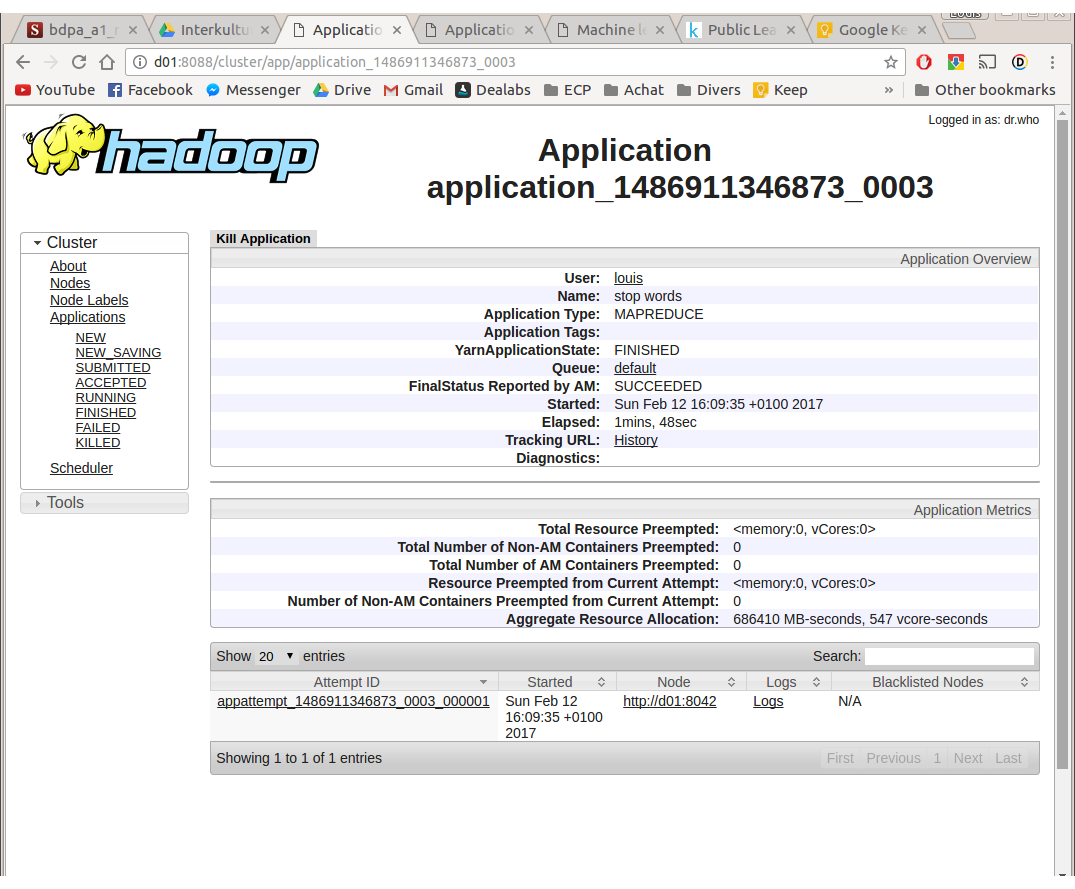
\includegraphics[width=.6\textwidth]{stopwords_10_reducers_1_combiner_compression.png}
\end{figure}

\subsubsection{(5) Run the same program again, this time using 50 reducers. Report the
execution time. Is there any difference in the execution time, compared to
the previous execution? Why?}
The running time with 50 reducers, combiner and compression is \textbf{126 seconds}.
The running time is about the same as the previous experiment.
We did not benefit from the additional number of reducers.
This is logical because with a single node cluster, the processing power caps with
the limited number of cores. No additional gain is achieved with this extra parallelization.
\begin{figure}[H]
  \centering
  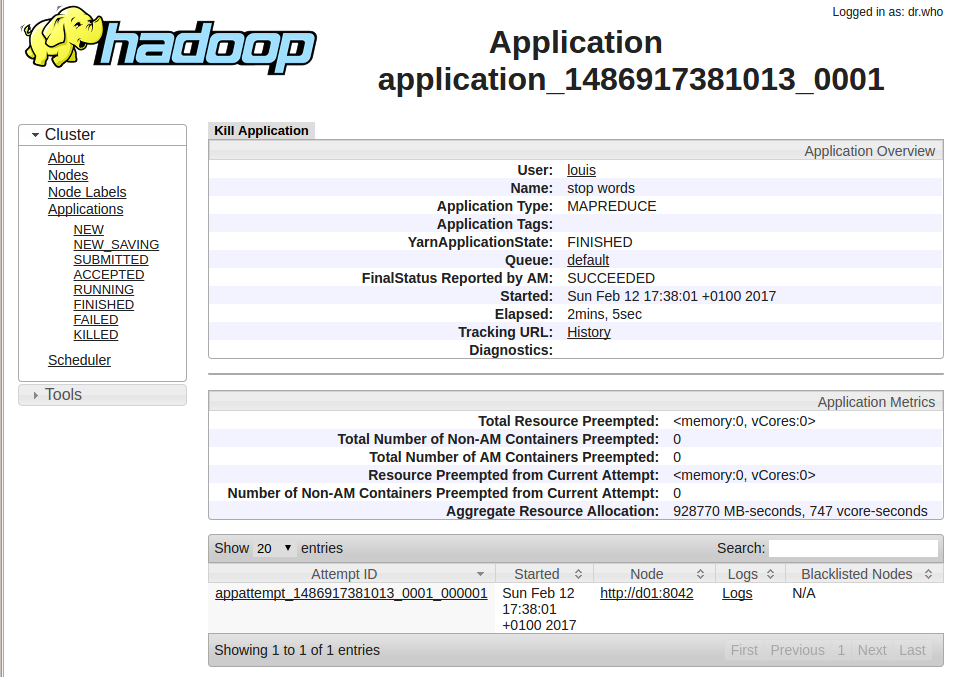
\includegraphics[width=.6\textwidth]{stopwords_50_reducers_1_combiner_compression.png}
\end{figure}


\subsection{(30) Implement a simple inverted index for the given document corpus, as shown in
the previous Table, skipping the words of stopwords.csv.}
The inverted index is implemented in \textbf{InvertedIndex.java}.
\begin{itemize}
  \item \textbf{readStopWords function:}\\
  First we need to read the stopwords from the csv file. We do it with the readStopWords function.
  \lstinputlisting[firstnumber=52, firstline=52, lastline=84, language=java]{assets/code/InvertedIndex.java}

  \item \textbf{Mapper:}\\
  Our mapper here outputs only words which are not in stopwords.csv as keys and
  the file from which they came from as values (formatted as a posting list).
  These posting lists are implemented using a custom class of MapWritable in order
  to have all the ComparableWritable properties that Hadoop's MapReduce needs (more details below).
  The posting list returned by the mapper is just a map containing one element
  which is a (key, value) pair of the form (filename, 1).
  \lstinputlisting[firstnumber=87, firstline=87, lastline=116, language=java]{assets/code/InvertedIndex.java}

  \item \textbf{Reducer:}\\
  Our reducer reduces all the posting lists it receives and also counts the number
  of occurences of each word for the following frequency part (more details below).
  \lstinputlisting[firstnumber=124, firstline=124, lastline=147, language=java]{assets/code/InvertedIndex.java}
\end{itemize}

\subsection{(10) How many unique words exist in the document corpus (excluding stop words)?
Which counter(s) reveal(s) this information? Define your own counter for the number
of words appearing in a single document only. What is the value of this counter? Store
the final value of this counter on a new file on HDFS.}
The counter that counts the unique words in the documents is \textbf{TaskCounter.REDUCE\_INPUT\_GROUPS}.
This counter counts the number of keys which is exactly the number of unique words.

In order to count the words appearing in a single document only, we implement the following counter:
\lstinputlisting[firstnumber=31, firstline=31, lastline=33, language=java]{assets/code/InvertedIndex.java}
Which is incremented in the reducer's reduce function:
\lstinputlisting[firstnumber=160, firstline=160, lastline=166, language=java]{assets/code/InvertedIndex.java}

The counter gives us a count \textbf{36343 words appearing in a single document only}
which seems pretty high given the number of total unique words 56491
(excluding about 140 stopwords).

After investigation, a lot of words appear only in pg3200.txt which are the Mark Twain works.
This file is roughly 300.000 lines long, which is about three times longer than the other files.
This might explained why it contains a lot more vocabulary specific than the rest.

The counter value is stored in a file in HDFS:
\lstinputlisting[firstnumber=220, firstline=220, lastline=227, language=java]{assets/code/InvertedIndex.java}

\subsection{(30) Extend the inverted index of (b), in order to keep the frequency of each word for
each document. You are required to use a Combiner.}
\begin{itemize}
  \item \textbf{PostingListWritable:}\\
  As explained before we implemented a custom class extending MapWritable in order to have
  all the ComparableWritable properties that hadoop needs and to be able to use a
  combiner along with a reducer without losing the word frequencies during the transfer.
  The custom class allows pretty printing a MapWritable instance to a file.
  \lstinputlisting[firstnumber=36, firstline=36, lastline=49, language=java]{assets/code/InvertedIndex.java}
  \item \textbf{Combiner:}\\
  Different posting lists coming from different mappers or combiners can be reduced
  into a single one using the reduce function of the combiner.
  \lstinputlisting[firstnumber=119, firstline=119, lastline=147, language=java]{assets/code/InvertedIndex.java}
  \item \textbf{Reducer:}\\
  The reducer shares the reduce function (it is a child of the combiner) with the combiner with the only exception
  that it will increment the counter for words in unique documents (which should only occur
  once per key and therefore only in the reducer).
  \lstinputlisting[firstnumber=150, firstline=150, lastline=168, language=java]{assets/code/InvertedIndex.java}
  \item \textbf{Results}:
  Here is an extract of the output inverted index csv:
  \lstinputlisting[firstnumber=1741, firstline=1741, lastline=1756]{assets/code/invertedindex.csv}
\end{itemize}

\section{Conclusion}

Inverted indexes are widely used for text retrieval or for search engines for the
performance gain they provide.
Creating an inverted index can however be a computing power intensive task but
it can be highly parallelized.
Hadoop's MapReduce framework is a perfect candidate for parallelizing this kind
of task on a highly distributed cluster with no centralized data.

\end{document}
